\documentclass{article}

\usepackage{graphicx}
\usepackage{tikz}
\usepackage{tikzsymbols}
\usetikzlibrary{calc,patterns,shapes.geometric}
\pagestyle{empty}
\usepackage[margin=0pt]{geometry}
\geometry{papersize={14in,12in}}

\def\centerarc[#1](#2)(#3:#4:#5){\draw[#1] ($(#2)+({#5*cos(#3)},{#5*sin(#3)})$) arc (#3:#4:#5);}

\begin{document}
	\begin{figure}
		\centering
		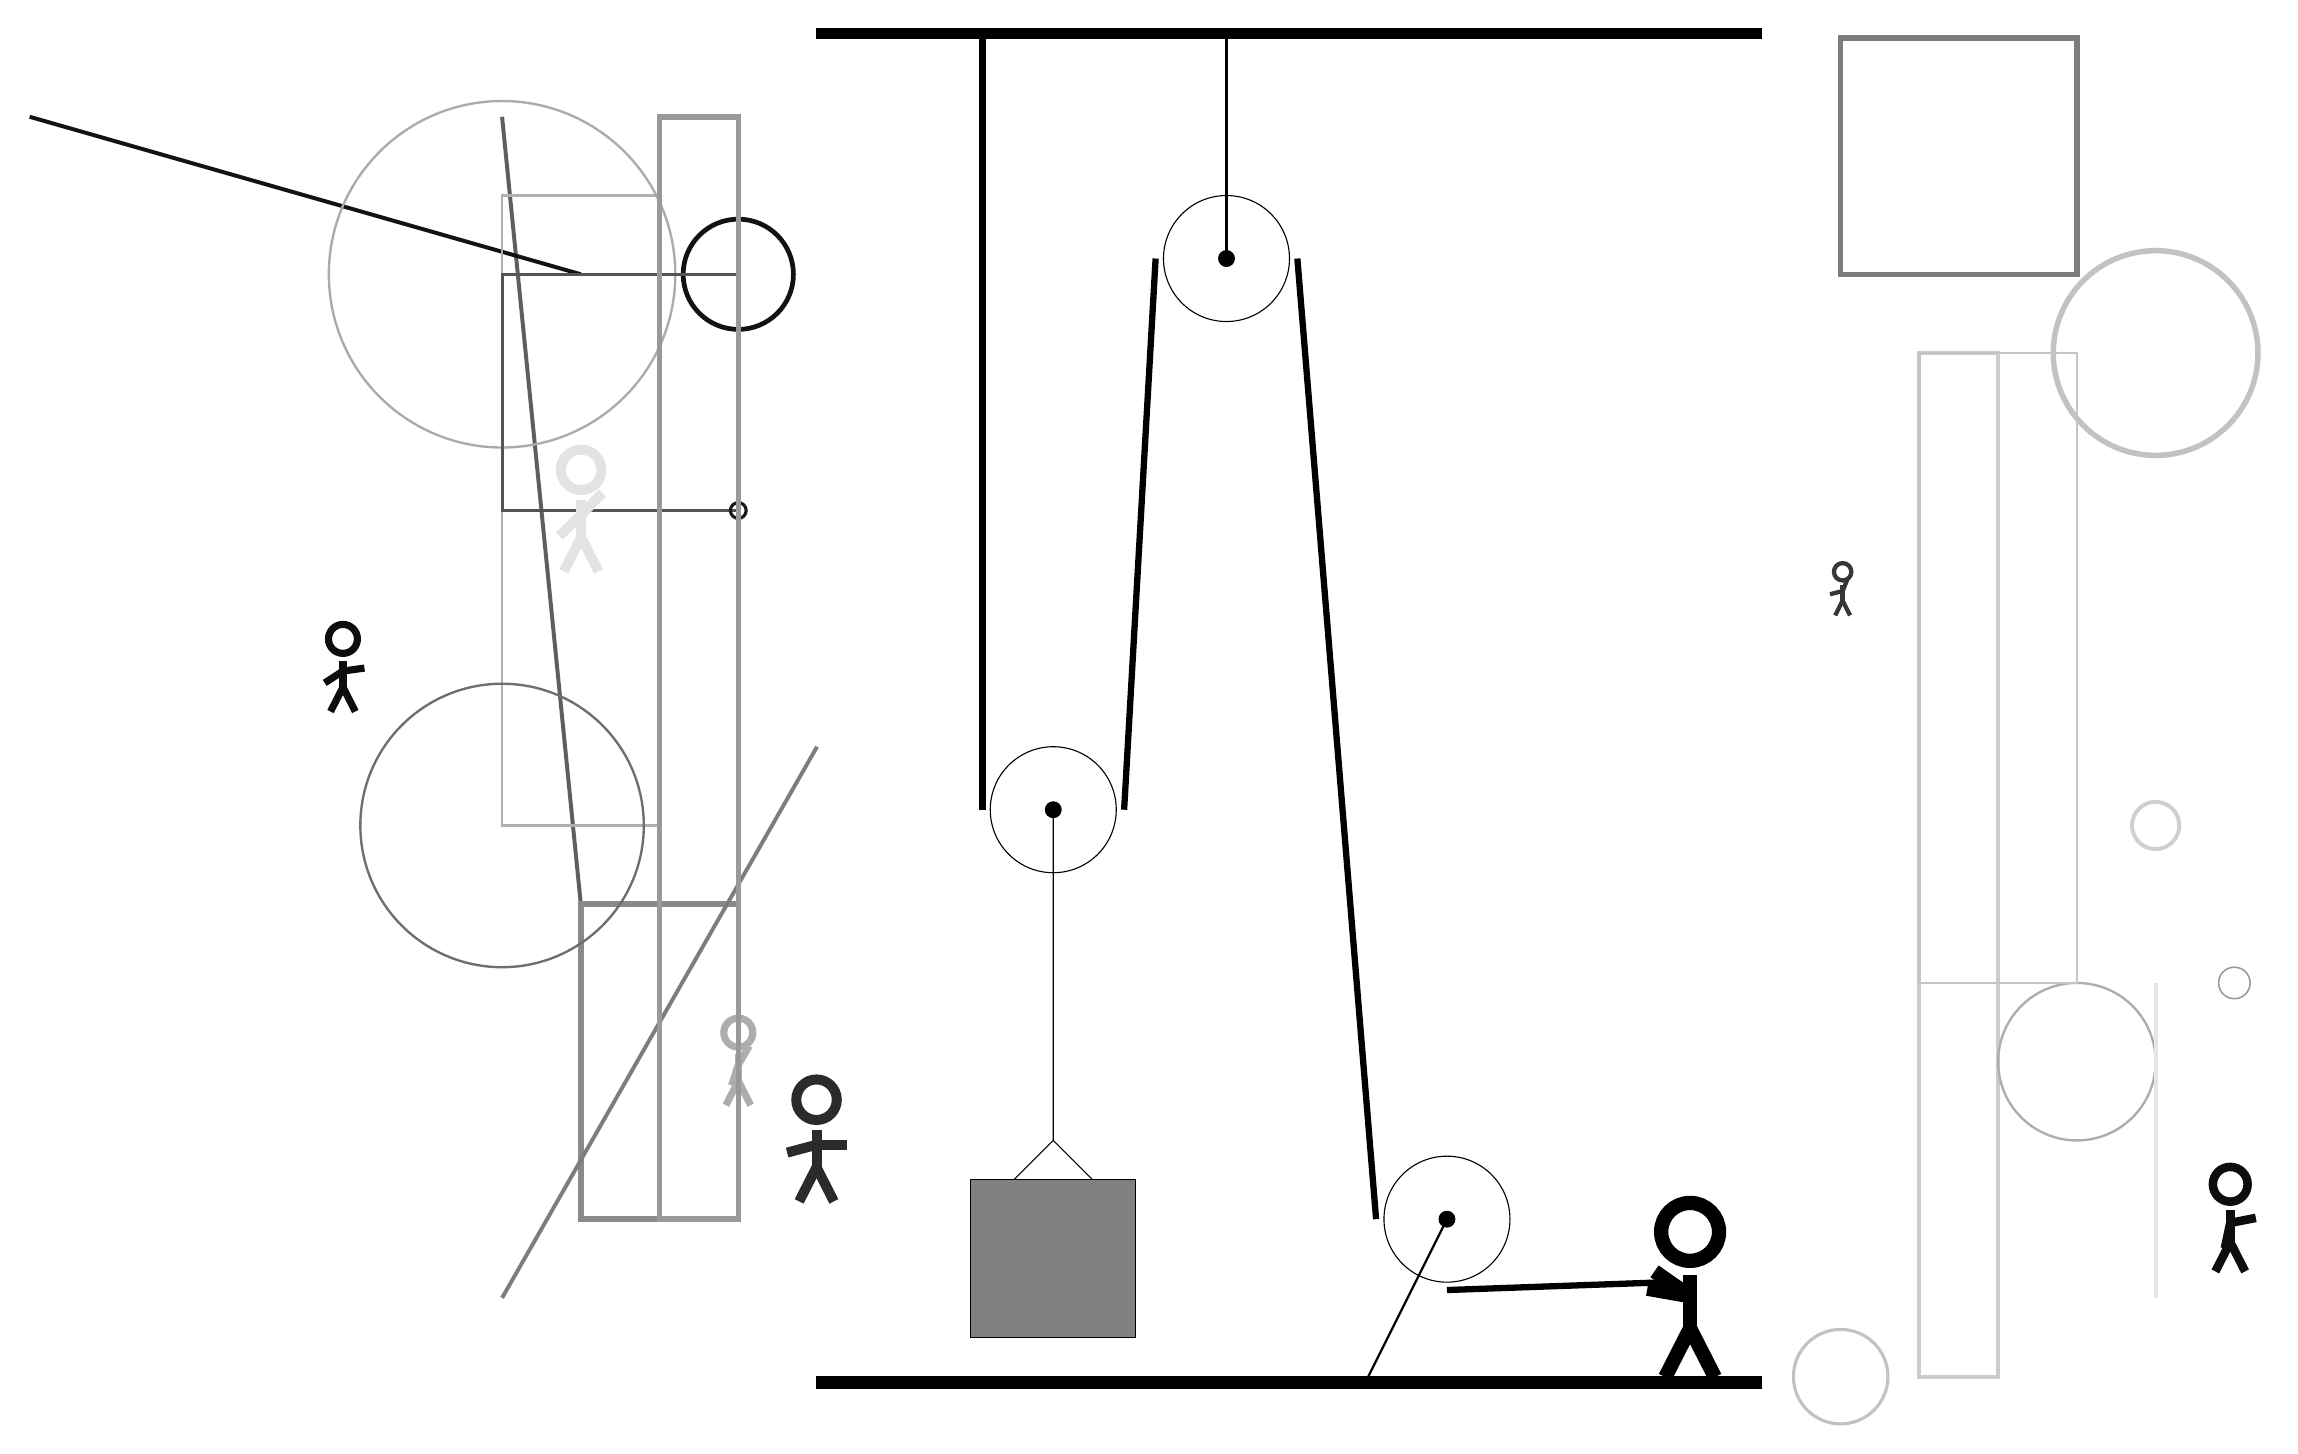
\begin{tikzpicture}
			%%%%% START %%%%%
			
			\draw[fill=black] (-2, 14) rectangle (10, 14.125);
			
			\draw (3.2, 11.2) circle (0.8);
			\draw[fill=black] (3.2, 11.2) circle (0.1);
			\draw[thick] (3.2, 11.2) -- (3.2, 14);
			
			\draw[line width=0.5mm, color=black!63](-5, 3) -- (-6, 13);
			
			\draw[line width=0.5mm, color=black!93](-5, 11) -- (-12, 13);
			\draw [line width=0.6mm, color=black!93](-3, 11) circle (0.7);
			\node[line width=0.3mm, color=black!95] at (-8, 6) {\Strichmaxerl[5][33][8]};
			\draw[line width=0.7mm, color=black!46] (-3, -1) rectangle (-5, 3);
			\node[line width=0.6mm, color=black!95] at (16, -1) {\Strichmaxerl[6][78][11]};
			\draw[line width=0.5mm, color=black!20] (12, -3) rectangle (13, 10);
			\draw [line width=0.3mm, color=black!32](14, 1) circle (1.0);
			\draw[line width=0.3mm, color=black!31] (-4, 4) rectangle (-6, 12);
			\draw[line width=0.5mm, color=black!10](15, 2) -- (15, -2);
			\draw [line width=0.3mm, color=black!57](-6, 4) circle (1.8);
			\draw[line width=0.3mm, color=black!23] (12, 10) rectangle (14, 2);
			\node[line width=0.7mm, color=black!79] at (11, 7) {\Strichmaxerl[3][14][68]};
			\draw [line width=0.2mm, color=black!40](16, 2) circle (0.2);
			\draw [line width=0.4mm, color=black!24](11, -3) circle (0.6);
			\draw[line width=0.5mm, color=black!51](-6, -2) -- (-2, 5);
			\draw [line width=0.3mm, color=black!33](-6, 11) circle (2.2);
			
			\draw[line width=0.4mm, color=black!67] (-3, 8) rectangle (-6, 11);
			\draw [line width=0.4mm, color=black!90](-3, 8) circle (0.1);
			\draw [line width=0.5mm, color=black!19](15, 4) circle (0.3);
			\draw [line width=0.7mm, color=black!24](15, 10) circle (1.3);
			
			\node[line width=0.3mm, color=black!32] at (-3, 1) {\Strichmaxerl[5][72][60]};
			\node[line width=0.2mm, color=black!11] at (-5, 8) {\Strichmaxerl[7][44][46]};
			\draw[line width=0.7mm, color=black!40] (-3, -1) rectangle (-4, 13);
			\draw[line width=0.7mm, color=black!51] (11, 14) rectangle (14, 11);
			
			\node[line width=0.3mm, color=black!83] at (-2, 0) {\Strichmaxerl[7][15][0]};
			
			\draw (6, -1) circle (0.8);
			\draw[fill=black] (6, -1) circle (0.1);
			\draw[thick] (6, -1) -- (5, -3);
			
			\draw (1, 4.2) circle (0.8);
			\draw[fill=black] (1, 4.2) circle (0.1);
			
			\draw (1, 4.2) -- (1, 0) -- (0.5, -0.5);
			\draw (1, 0) -- (1.5, -0.5);
			\draw[fill=black!50] (-0.05, -0.5) rectangle (2.05, -2.5);
			
			\draw[line width=0.8mm] (0.1, 14) -- (0.1, 4.2);
			\centerarc[line width=0.8mm](1, 4.2)(180:360:0.9);
			\draw[line width=0.8mm](1.9, 4.2) -- (2.3, 11.2);
			\centerarc[line width=0.8mm](3.2, 11.2)(0:180:0.9);
			\draw[line width=0.8mm](4.1, 11.2) -- (5.1, -1);
			\centerarc[line width=0.8mm](6, -1)(180:270:0.9);
			\draw[line width=0.8mm](6, -1.9) -- (8.8, -1.8);
			
			\node at (9, -1.9) {\Strichmaxerl[10][-35][170]};
			
			\draw[fill=black] (-2, -3) rectangle (10, -3.15);
			
			%%%%% END %%%%%
		\end{tikzpicture}
	\end{figure}	
\end{document}